\documentclass[preprint, journal=prl]{revtex4-1}
\usepackage{graphicx}
\usepackage{amsmath}
\usepackage{braket}
\usepackage{float}
\usepackage{caption}
\usepackage{color}


\begin{document}
\title{Numerical Determination of the Hartree-Fock Stability of the Paramagnetic Electron Gas in 1, 2 and 3 Dimensions}
\author{Evan Curtin}
\author{So Hirata}
\email{Sohirata@illinois.edu}
\affiliation{Department of Chemistry, University of Illinois at Urbana-Champaign, 600 South Mathews Avenue, Urbana, Illinois 61801, USA}

\begin{abstract}
  In molecular electronic structure theory, breaking symmetry of a Hartree-Fock reference serves as a viable means to resolve spurious degeneracies in certain systems. This allows for the use of a wide array of post-Hartree-Fock methods to recover more of the correlation energy. While there exists proofs of the existence of lower energy broken symmetry solutions under certain circumstance in the finite case, we are unaware of analogous ones in the periodic case. This study presents numerical experiments into stability of paramagnetic solutions of the Homogeneous electron gas within the Hartree-Fock approximation to glean insight into the periodic case. We show that in 2 and 3 dimensions, the paramagnetic solution is unstable at $r_s$ above 0.87 and 3.2 atomic units, respectively. In one dimension the solution is essentially always unstable, in agreement with Overhauser's theorem. This approach also lends itself to a means of finding lower energy broken symmetry solutions, at various levels of restriction within Hartree-Fock theory.
\end{abstract}

\maketitle

\section{Introduction}
  The goal of electronic structure theory is to solve the electronic Schr{\"o}dinger equation  for a molecule or solid state system. The prevailing approach in \emph{ab initio} quantum  chemistry is to first compute a self-consistent single-determinant Hartree-Fock (HF) solution which will serve as a reference for many-body perturbative (MP) or coupled-cluster (CC) approaches. Implicit in these methods is the assumption that the reference wave function will be sufficiently close to the exact solution of the Schr{\"o}dinger equation to converge to the correct answer in a computationally feasible manner. Both the MP and CC approaches have the attractive quality that they are systematically improvable, i.e. increasing the accuracy of the resulting solution can be done by using a higher order of the theory. These so-called post-Hartree-Fock methods are able to recover more of the total electronic energy by accounting for the \emph{correlation energy} in the system. Traditionally, the correlation energy is defined by the difference between the exact energy and the Hartree-Fock energy \cite{Shavitt2009}
  \begin{equation}\label{eq:correlation_energy}
    E_{corr} = E_{exact} -  E_{HF}.
  \end{equation}
  In many cases the correlation energy is relatively small and the Hartree-Fock reference captures a significant portion of the exact total energy. In such cases, the prevailing approach is usually successful and has only implementation issues for larger systems. On the other hand there are systems which are not well treated by this approach, which are often called ``strongly correlated''. Examples of such systems are those with degenerate or near-degenerate HOMO-LUMO gaps, metallic solids or molecules close to breaking bonds. Oftentimes for such systems the traditional Hartree-Fock solutions are not even qualitatively correct, implying inadequacies in either the single-reference or mean-field approach.    
  
  It is often neglected, however, that the usual way for computing a Hartree-Fock solution in practice is to use a restricted form of the single determinantal wavefunction. In the Restricted  Hartree-Fock (RHF), the wave function is restricted to be an eigenfunction of the $\hat{S^2}$ and $\hat{S_z}$ operators, while in the Unrestricted variant (UHF), the wave function need only be an eigenfunction of the $\hat{S_z}$. There is yet another lesser-known variation of the theory, known as General Hartree-Fock (GHF), which assumes no spin-symmetries in the wave function. This allows for greater variational flexibility at the cost of ``broken symmetry''. Together these three levels of Hartree-Fock theory form a heirarchy of increasing parameter space within which to minimize the total energy. In order to test whether or not a lower energy solution of broken symmetry exists, a ``stability analysis'' can be performed on a determined Hartree-Fock solution. 
  
  First, a self-consistent solution to the HF equations needs to be found, but being a solution to the Hartree-Fock equation ensures only that the solution is stationary with respect to the determined orbitals. If the solution is indeed a minimum, it is called ``stable'', while if there is any displacement in the electronic structure which lowers the energy, the solution is ``unstable''. A method for determining the stability of a Hartree-Fock solution was proposed by Thouless in 1960\cite{Thouless1960}. The condition was rederived into the expression familiar to quantum chemists by Čížek and Paldus in 1967\cite{Cizek1967}. Furthermore, the stability equations factorize depending on the symmetry of the Hartree-Fock eigenfunctions. To this end, Seeger and Pople outlined a hierarchical approach to systematically evaluate the stability of HF states in the restricted, unrestricted and generalized Hartree-Fock procedures\cite{Seeger1977}. Recently, the method has been used to aid the search for the lowest-energy Unrestricted Hartree-Fock (UHF) solutions in molecules, as well as the General Hartree-Fock (GHF) solutions in geometrically frustrated hydrogen rings which cannot conform even to the UHF scheme\cite{Pulay2016, Goings2015}. The lower energy HF solutions in these studies were located by first finding the instabilities in the higher spin-symmetry solutions, then using this information to obtain ``symmetry breaking'' displacements that lower the energy.    
    
  Previously it has been shown for finite systems with form-degenerate HOMO-LUMO, there always exists a symmetry-breaking instability\cite{Yamada2015}. Whether this theorem holds in the infinite case remains to be seen. To investigate HF instabilities in zero band gap solids, a natural starting point is the Homogeneous Electron Gas (HEG, often called Jellium or Uniform Electron Gas) model. The model consists of electrons in a box with periodic boundary conditions  and the constraint that the entire system is charge-neutral via a uniform background positive  charge. The resulting Coulomb interactions cancel exactly, and the only remaining terms are due   to kinetic and exchange energies. Historically it was thought that the plane-wave paramagnetic solution to the HF equations for this model was the ``correct'' solution. However, in a landmark paper, Overhauser showed that certain symmetry broken solutions \emph{always} have lower-energy than the paramagnetic solutions at all electron densities\cite{Overhauser1962}. This hints at, but does not show, that the analogous triplet instability theorem persists in the infinite case.  
        
  Overhausers' paper sparked new interest in the HEG, and since then Energies of various phases thereof have been computed to great accuracy\cite{Ceperley1980}. More recently, phase diagrams have been determined for the HEG in 2 and 3 dimensions\cite{Delyon2008, Bernu2011, Baguet2013}. In all cases the phase diagrams are made by computing the energies of the polarized and unpolarized states, and comparing them. This approach necessitates that the form of the solutions is known ahead of time. 
  
  The present work focuses on directly calculating the Hartree-Fock stability of the paramagnetic homogeneous electron gas as a function of electron density. The motivation is two-fold. First, the numerical studies of this model can give computational evidence for or against the ubiquity of symmetry-breaking HF instabilities in metallic solids. Secondly, the instabilities can help in determining lower energy HF solutions of the HEG. This is because the study will reveal where the symmetry broken Hartree-Fock reference is needed. To date, an optimal form (i.e. minimal energy in the HF manifold) of the Hartree-Fock solution to the HEG remains unknown, even though exact energy (including correlation) is essentially known. Therefore determining a lower energy HF solution can yield insight into the effects of correlation of this fundamental physical model.
        
 % Thus the term ``Hartree-Fock Energy'' is inherently ambigious; this fact calling into question commonly held ideas about correlation and Hartree-Fock theory. Take for example the dissociation curve of H$_2$ in the RHF and UHF approximations, compared with the exact solution obtained by full configuration-interaction in the complete basis set limit.   
 % \begin{figure}[H]
 %   \centering
 %   \includegraphics[width=0.75\textwidth]{../../images/H2_curves.eps}
 %   \caption{Dissociation curve of H$_2$ in the RHF and UHF approximations, compared to the exact limit (FCI). The difference in correlation energies as determined by each reference illustrates the ambiguity of that quantity. In the dissociation limit, the UHF correlation energy vanishes while the RHF correlation energy increases in magnitude.}
 %   \label{h2diss}
 % \end{figure}
 % The correlation energy for the RHF reference case is dramatically larger than that for the UHF reference. In other words, \emph{the correlation energy is, by definition, inherently coupled to the Hartree-Fock reference}. The given example is well understood, but it brings to mind a more general idea that there may be more cases where apparently large correlation energies are due to simply using and inadequate level of Hartree-Fock theory. Scuseria and coworkers have leveraged this idea to create new coupled cluster theories while preserving the symmetry of the reference  \cite{Gomez2016}. 
  
  %Another approach to this problem is to allow breaking of symmetry, and to take the variational principle at face value; lower energy is always better. For predicting certain observables this is not the case, but for energies alone we are free to maintain this mindset. If the HF solution is allowed to relax fully in its most general form, the resulting correlation energy may be reduced dramatically. Therefore the overarching theme of the proposed work is that \emph{many examples of strong correlation may be misleading, and in order to find out we have to find lower  energy Hartree-Fock solutions, even at the cost of broken symmetry}.
    
  %If it turns out that fully minimizing the HF energy can reproduce a majority of the ``correlation energy'' in these systems, then using this HF searching method becomes a justified method of solving strongly correlated systems. This would mean that the strong correlation was in fact illusory, and is convertible to a weak correlation problem by means of a more rigorous Hartree-Fock theory.
    
\section{Method}

  
  To determine if there is indeed a symmetry-broken HF solution of lower energy, the usual method  is to determine the stability of a found Hartree-Fock solution. Instabilities are indicated by a negative eigenvalue in the Electronic Hessian, 
  \begin{equation}
    \bf{H}=
    \begin{bmatrix}
      \bf{A} &\bf{B} \\
      \bf{B}^* & \bf{A}^* \\
    \end{bmatrix},
  \end{equation} 
  where the matrices $\mathbf{A}$ and $\mathbf{B}$ have dimension $N_{occupied} \times N_{virtual}$ with elements given by
  \begin{align}
     A_{i \rightarrow a, j \rightarrow b} &= (\epsilon_a-\epsilon_i)\delta_{ij}\delta_{ab} 
     + \left< aj||ib \right>, \\
     B_{i \rightarrow a, j \rightarrow b} &= \left< ab||ij \right>. 
  \end{align}    
  
  Where occupied states are labelled by $i$ and $j$, virtual by $a$ and $b$, and $i \rightarrow a$ refers to the excitation which replaces state $i$ with state $a$. The relevant two electron notation is
  \begin{equation}
    \left< pq||rs \right> = \left< pq|rs \right> - \left< pq|sr \right>,
  \end{equation}
  where, 
  \begin{equation}
    \left< pq|rs \right> = \int \int \phi^*_p(\vec{r}_1) \phi^*_q(\vec{r}_2) \frac{1}{r_{12}} \phi_r(\vec{r}_1) \phi_s(\vec{r}_2) d\vec{r_1} d\vec{r_2}, 
  \end{equation}
  and states labeled with $p$, $q$, $r$, or $s$ are either occupied or virtual. For a paramagnetic HF solution (RHF), the Orbital Hessian factorizes into the matrices known to chemists as the singlet and triplet instability matrices ($\bf{{}^1H}$ and $\bf{{}^3H}$, respectively)\cite{Dunning1967,Seeger1977}.
  \begin{subequations}
    \begin{eqnarray}
      {}^{1}{A'}_{i\rightarrow a, j\rightarrow b} &=& 
      (\epsilon_a-\epsilon_i)\delta_{ij}\delta_{ab} 
      + 2\braket{aj|ib}-\braket{aj|bi}\\
      {}^{3}{A'}_{i\rightarrow a, j\rightarrow b} &=& 
      (\epsilon_a-\epsilon_i)\delta_{ij}\delta_{ab} 
      - \braket{aj|bi}\\
      {}^{1}{B'}_{i\rightarrow a, j\rightarrow b} &=& 2\braket{ab|ij}-\braket{ab|ji}\\
      {}^{3}{B'}_{i\rightarrow a, j\rightarrow b} &=& -\braket{ab|ji}
    \end{eqnarray}
  \end{subequations}
  The lowest eigenvalue of both of these matrices will reveal the stability of the RHF solution. If  ${}^1\bf{H}$ has negative eigenvalues, the solution is unstable with respect to changes that preserve singlet character (singlet instability), while if ${}^3\bf{H}$ has negative eigenvalues, the solution is unstable towards displacements that would change the wavefunction towards a triplet state (triplet instability). The solution is stable if neither ${}^1\bf{H}$ nor ${}^3\bf{H}$ has a negative eigenvalue. An eigenvalue of 0 does not indicate instability, and this case is discussed in detail by Cui et al \cite{Cui2013}.   
    	
  To apply the stability analysis to the electron gas, start with the Jellium Hamiltonian in atomic units, 
  \begin{equation}\label{hamiltonian}
   	\hat{H} = \sum_i \frac{\hat{p}_i^2}{2}  + \frac{1}{2} \sum_{i < j} \frac{1}{|\vec{r}_i - 
   	\vec{r}_j|}.
  \end{equation}
  One solution to the Hartree-Fock equations in $D$ dimensions are plane waves of the form	
  \begin{equation}\label{planewave}
   	\phi_{\vec{k}} =
    \frac{1} { \sqrt{L ^ D} } e ^ {i \vec{k} \dot \vec{x}},
  \end{equation}
  where $L$ is the length of one side of the direct lattice with cubic symmetry. Using this as the basis for the rest of the analysis, the two electron repulsion integrals are analytic and  well-behaved in two and three dimensions\cite{Delyon2008, Guiliani2005}
  \begin{align}
    \braket{\vec{k}, \vec{k}' | \vec{k}'', \vec{k}'''} 
    \stackrel{ \text{2D, 3D} }{=}&
    \begin{cases} 
      \frac{\pi} {L ^ D} \frac{ 2^{D-1} } { | \vec{k} - \vec{k}'' | ^ {D-1} } 
      & \vec{k}''' = \vec{k} + \vec{k}' - \vec{k}'' + n\vec{G} \textbf{ and } | \vec{k} - 
      \vec{k}''| \neq 0 \\
      0 
      & \text{else},
    \end{cases}
  \end{align}
  where $n\vec{G}$ is any integer times a reciprocal lattice vector of the system. The orbital energies are
  \begin{equation}\label{eq:hf_orb_energy}
    \epsilon_{\vec{k},\sigma}=
    \frac{\hbar^2\vec{k}^2}{2m} - \sum\limits_{\vec{k}}^{|\vec{k}|< 
    k_f}n_{\vec{k}\sigma}\braket{\vec{k}, \vec{k}' |\vec{k}', \vec{k}},
  \end{equation}
  where $n_{\vec{k}\sigma}$ is the occupation number of the state with momentum $\vec{k}$ and spin $\sigma$ \cite{Guiliani2005}. In one dimension, the two electron integral diverges, and it is common to use a delta function interaction, 
  \begin{equation}
    V(r_{12}) = V_0\delta(r_{12}),
  \end{equation}
  and the two electron integral in this case is simply
  \begin{align}\label{eq:ERI_1d}
    \braket{\vec{k}, \vec{k}' | \vec{k}'', \vec{k}'''} 
    \stackrel{ \text{1D} }{=}&
    \begin{cases} 
      V_0 
      & \vec{k}''' = \vec{k} + \vec{k}' - \vec{k}'' + n\vec{G}\\
      0 
      & \text{else}.
    \end{cases}
  \end{align}  
  These expressions can be used to evaluate the stability of the paramagnetic electron gas. In doing so, presence of instabilities of triplet (${}^3\mathbf{H}$) character are a sufficient, but not necessary, condition that a solution with different densities of $\alpha$ and $\beta$ spin exists which has lower energy than the paramagnetic solution. An example of such a solution would be the spin-density-wave (SDW) solution. 
   
\section{Results}   
  Using the equations for energies and two electron integrals, the stability analysis was performed on the paramagnetic HEG model as a function of electron density (or equivalently, the Wigner-Seitz radius, $r_s$). The approach of explicitly constructing and diagonalizing the orbital hessian is intractable both in terms of memory and calculation time requirements. Since the instability condition is that the any eigenvalue is negative, it suffices to calculate the sign of only the lowest eigenvalue. This is a task well suited for an iterative subspace solver. To this end, the Jacobi-Davidson algorithm was from the SLEPc library was used to calculated the lowest eigenvalues using the Blue Waters Supercomputer\cite{Hernandez2005}. 
  
  A basis of plane waves with simple cubic symmetry was used for all calculations, and the number of k-points was incremented until the lowest eigenvalues were sufficiently converged {\color{red} (for 1D and 2D more data can be gathered but in 3D getting more data is computationally unfeasible at the moment)}. In the 1D calculations, a potential of $V_0 = 1$ in atomic units was used.
  \begin{figure}[H]
    \centering
    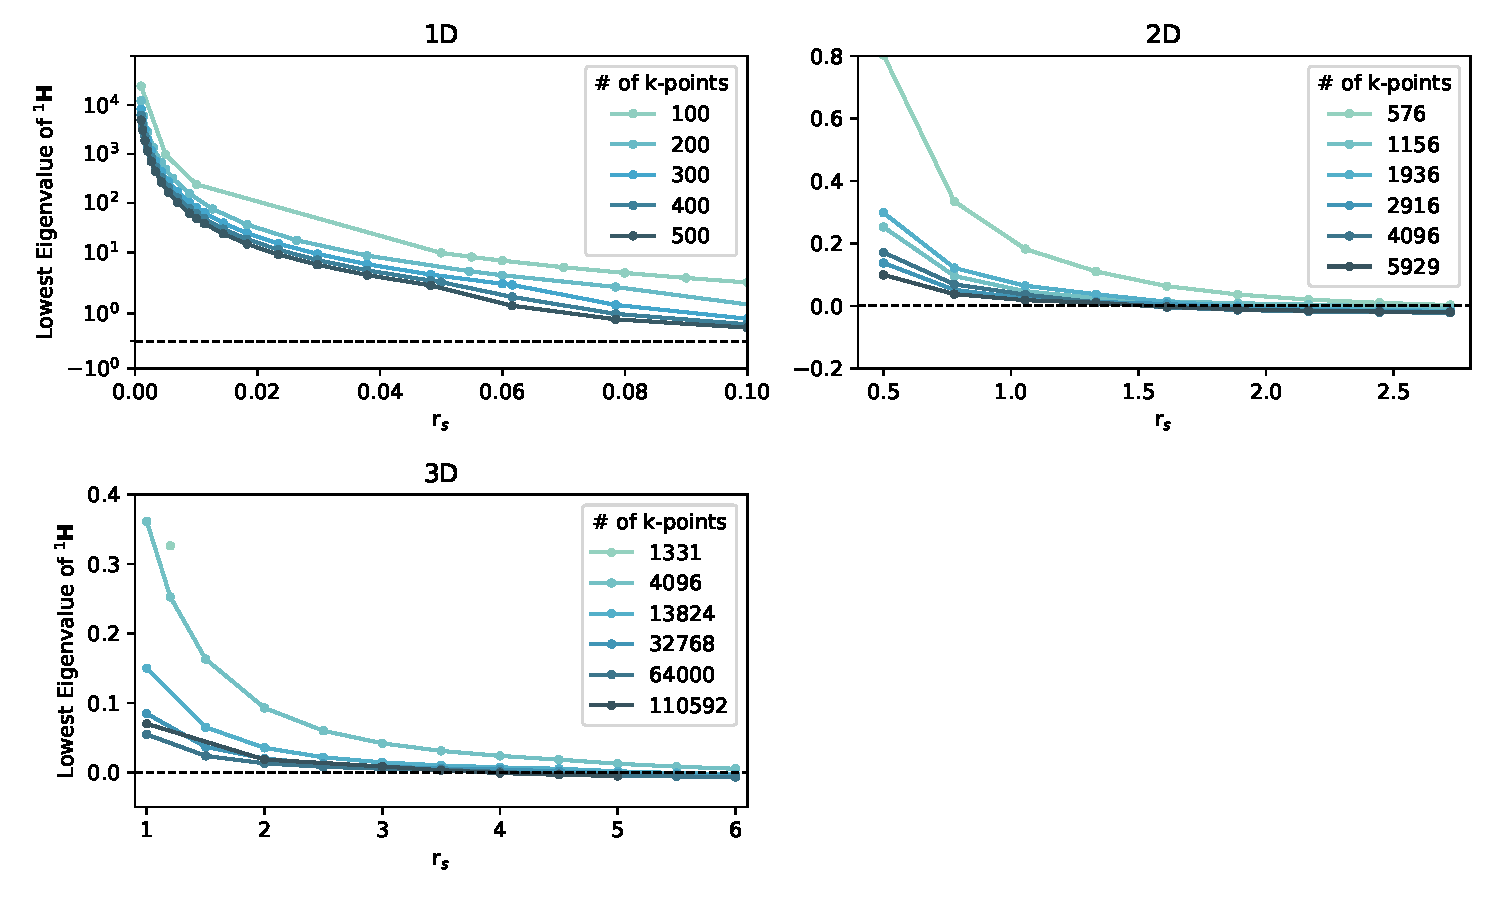
\includegraphics[width=\textwidth]{../../images/singlet-stability-convergence.eps}
    \caption{The lowest eigenvalue of ${}^1\mathbf{H}$ as a function of $r_s$ with increasing number of k-points in 1, 2 and 3 dimensions.}
    \label{fig:singlet_convergence}
  \end{figure}
  \begin{figure}[H]
    \centering
    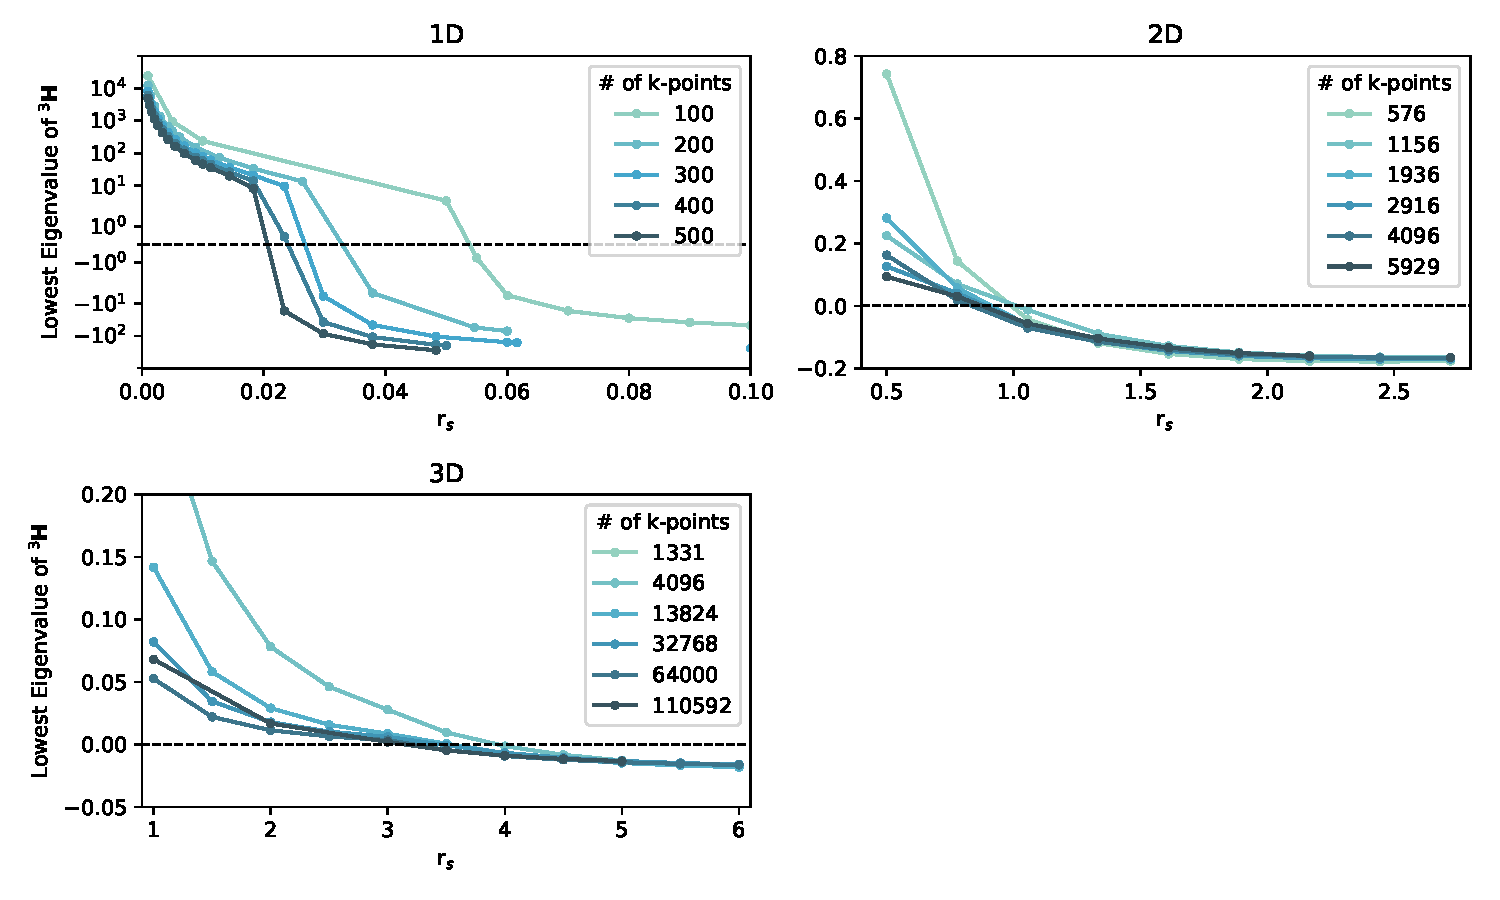
\includegraphics[width=\textwidth]{../../images/triplet-stability-convergence.eps}
    \caption{The lowest eigenvalue of ${}^3\mathbf{H}$ as a function of $r_s$ with increasing number of k-points in 1, 2 and 3 dimensions.}
    \label{fig:triplet_convergence}
  \end{figure}
  To determine the $r_s$ at which the lowest eigenvalue of $\mathbf{H}$ changes sign, the lowest eigenvalues were linearly interpolated  {\color{red} (this can easily be changed to one of [(‘linear’, ‘nearest’, ‘zero’, ‘slinear’, ‘quadratic’, ‘cubic’ where ‘zero’, ‘slinear’, ‘quadratic’ and ‘cubic’ refer to a spline interpolation of zeroth, first, second or third order)]} as a function of $r_s$ and solving
  \begin{equation} \label{eq:transition_rs}
    \lambda_{min}(r_s) = 0.
  \end{equation}
  The solution to eq. \ref{eq:transition_rs} is referred to as the transition $r_s$ and this quantity was determined while increasing the number of k-points in the simulation to convergence (see Fig. \ref{fig:onset}).
  \begin{figure}[H]
    \centering
    \includegraphics[width=\textwidth]{../../images/combined_onset.eps}
    \caption{The value of $r_s$ at which the singlet (green) and triplet (blue) instability    occurs with increasing number of k-points in 1, 2 and 3 dimensions. In the 1D case (left), the singlet instability never appeared in the calculations performed. }
    \label{fig:onset}
  \end{figure}
  
  
  \begin{table}[H]
  \centering
  \caption{The values of $r_s$ at which the lowest eigenvalue of $\mathbf{H}$ changes sign.}
    \begin{tabular}{ c | c }
      D~~~ & ~~ Transition $r_s$ (bohr$^{-1}$) \\
      \hline
      1    &  0.02 \\
      2    &  0.87 \\
      3    &  3.16 \\
      \hline
     \end{tabular}
  \label{table:transition_rs}
  \end{table}  
  The transition $r_s$ values are presented in table \ref{table:transition_rs}. These results are consistent with those seen by other methods, which show the emergence of broken symmetry phases with distinguishably lower energy at $r_s \approx 0.8$ in 2D and $r_s \approx 3$ in 3D\cite{Baguet2014, Bernu2011}. On the other hand, the transition $r_s$ for one dimension tends towards zero and stays quite close as the number of grid points increases. Indeed, numerical issues appear at very high density (low $r_s$) due to divergence of the two electron integrals in the asymptotic limit. With this in mind, it is clear at least that the instability in the 1D case persists even at very high densities (potentially all finite densities), which is to be expected from Overhauser's proof of instability at all values of $r_s$ in 1D for the delta function potential \cite{Overhauser1962}.

  
\section{Conclusion}
  The paramagnetic Hartree-Fock solution to the Homogeneous electron gas was shown numerically to be unstable with respect to broken symmetry solutions at certain densities, which were determined in 2 and 3 dimensions. The one dimensional solution with the delta function potential is effectively always unstable (that is to say, the value of $r_s$ at which the solution becomes unstable is within numerical error of zero). These results are compatible with Overhauser's theorem and direct energy comparisons. While the present study did not find lower energy broken symmetry solutions, the procedure for doing so is outlined by Seeger\cite{Seeger1977}. This procedure may be computationally difficult to actualize for this system, but nevertheless could be a worthwhile pursuit. By tracing the instability eigenvectors downhill in energy, the broken symmetry solutions of lower energy may be found. Since the correlated energy is known, it could be compared to the lowest energy Hartree-Fock energy found and may give insights into the ability of broken symmetry Hartree-Fock solutions to describe periodic systems. 

  
\begin{acknowledgements}
The authors would like to thank...
\end{acknowledgements}

\section{References}
\bibliography{references}

\end{document}